%Archivo latex del proyecto final

%Formato artículo, tamaño de letra 11
\documentclass[11pt,a4paper]{article}


%Todos estos paquetes son los que he usado en el tfg
%Sé que hay muchos, pero por si acaso los pongo
\usepackage[utf8x]{inputenc}
\usepackage{array}
\usepackage{amsmath}
\usepackage{amsbsy}
\usepackage{bm} %Para poner en negrita las letras griegas, tambien sirve el de arriba
\usepackage{upgreek} %Para quitarle la cursiva a las letras griegas, con el comando \up''letra griega'' todo junto
\usepackage{mathrsfs} 
\usepackage{amssymb}
\usepackage{marvosym}
\usepackage{epsfig}
\usepackage{graphics}
\usepackage{graphicx}
\usepackage{amsfonts}
\usepackage{xspace}
\usepackage{color}
\usepackage{booktabs}
\usepackage{xtab}
\usepackage{subfig}
\usepackage{graphicx}

\usepackage[spanish]{babel}

\begin{document}

\title{\'Atomos Ultrafr\'ios}
\author{Jos\'e Ponce Chulani}

\maketitle


\bigskip

\begin{abstract}
  %URL del repositorio
  En este artículo vamos a tratar brevemente un campo de la física cuántica que está en auge: el de los \'atomos y m\'oleculas ultrafr\'ias. Nos centraremos en el modelo de Bose-Hubbard para estudiar algunas de sus propiedades. Estudiamos casos concretos de la ecuación de Schroedinger independiente y dependiente del tiempo. Vemos como la dinámica depende de las simetrías del sistema y de la función de onda inicial.
\end{abstract}

\bigskip

\textit{Palabras Clave:}
Átomos ultrafríos, modelo Bose-Hubbard, superfluido, aislante Mott, tuneleo.

\newpage 

\begin{abstract}
  %URL del repositorio
  In the current proyect we give a brief review of an investigation field of quantum physics that is very popular nowadays: the ultracold atoms or molecules. Specifically we study some properties of the Bose-Hubbard model. We study specific systemsforthe time independent and dependent Schroedinger equation. We demonstrate that the dynamic's system depends on the Hamiltonian symmetries and on the initial wave function.
\end{abstract}

\bigskip

\textit{Keywords:}
Ultracold atoms, Bose-Hubbard model, suprfluid, Mott insulattor, tunneling.

\newpage

\section{Introducción}

Sabemos que en física cuántica hay dos tipos de partículas: los bosones y fermiones. Con espines entero y semientero respectivamente, su propiedad fundamental es que pueden existir todos los bosones que queramos en el mismo estado cuántico mientras que los fermiones no. Por tanto esperaremos encontrar propiedades y estados bosónicos curiosos. También sabemos que toda partícula masiva lleva asociada una longitud de onda, y que, a mayor longitud de onda mayores efectos cuánticos podremos observar. Así, necesitaremos temperaturas realmente frías para que la longitud de onda de las partículas sean lo suficientemente altas como para encontrar efectos cuánticos.

En este  trabajo

%CREO QUE ESTO ES EL ESTADO DEL ARTE
\textir{Estado del arte}

Este tipo de redes son muy versátiles: se pueden conseguir muchas geometrías diferentes casi sin defectos, e incluso puede cambiarse su forma y la intensidad de los mínimos de potencial en el curso de un experimento. 


\section{El sistema}

Como ya hemos mencionado nuestro modelo contiene dos ingredientes básicos: una red óptica y una cierta cantidad de átomos que vamos a cargar en la red. Estos átomos van a ser de carácter bosónico, de manera que tendremos la libertad de almacenar tantos como queramos (o cuanto podamos, mejor dicho) en un mismo estado cuántico. La dinámica de los bosones a lo largo de la red va a depender de dos términos fundamentalmente, la energía cinética de los átomos y de cuán fuerte interaccionen entre ellos, pudiendo dar lugar al famoso efecto túnel cuando la primera energía domine sobre la otra.



La red óptica se logra haciendo interferir dos rayos láser, formando un patrón de pozos potenciales. En este patron se carga el gas de bosones ya enfriado, de manera que un esquema del sistema viene dado por la figura \ref{f:red}.

\begin{figure}[h]
  \centering
  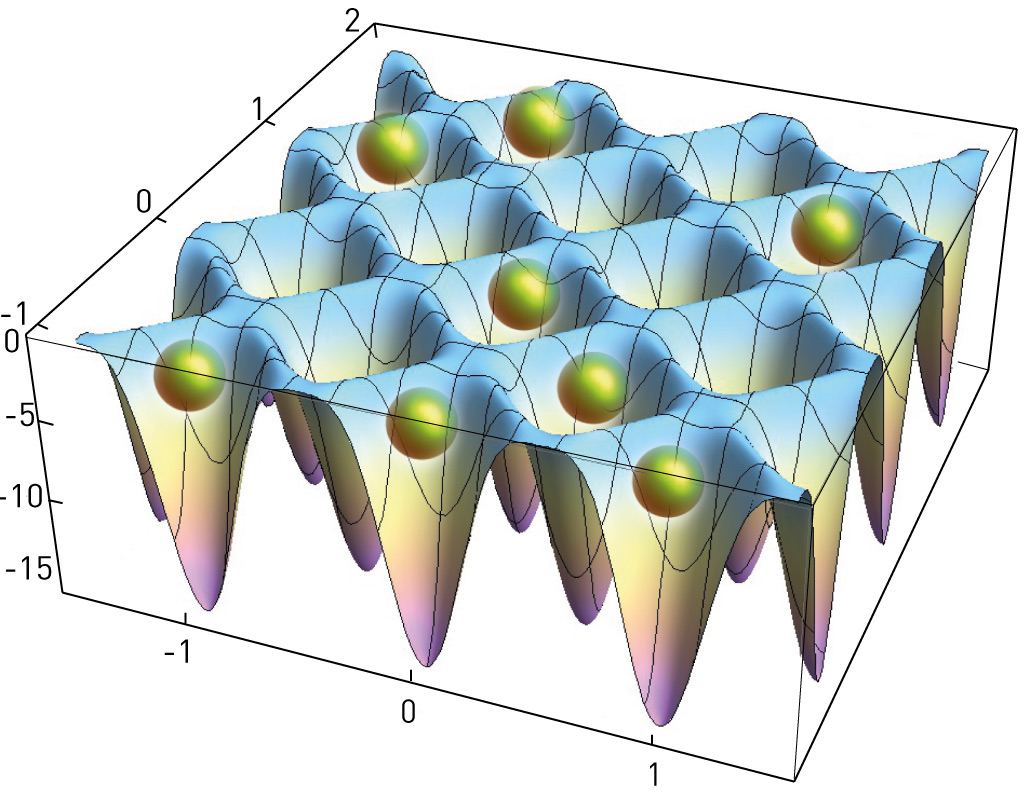
\includegraphics[width=8cm]{hi_8148.jpg}
  \caption{Esquema de una red óptica bidimensional con átomos en sus pozos potenciales.}
  \label{f:red}
\end{figure}
\noindent

De esta figura también puede verse que es el mismo concepto que las redes cristalinas en física del estado sólido. Por tanto, usaremos las funciones de Bloch para describir a nuestros bosones descolalizados en la red, recordemos que, para un espaciado de la red $a$, las soluciones de la ecuación de Schroedinger vienen dadas por

\begin{equation}
  \begin{split}
    & \phi^{(n)}(x)=\textit{e}^{iqx}u_q^{(n)}(x) \\
    & u_q^{(n)}(x+a)=u_q^{(n)}
  \end{split}
\end{equation}

donde q es el número de onda de la partícula y $u_q^{(n)}(x)$ es la función que contiene la perioricidad de la solución.



A partir de estas funciones se definen las conocidas funciones de Wannier, que se usan para localizar los átomos en un mínimo de potencial dado. Estas funciones se definen:

\begin{equation}
  \omega_n(x-x_j)=\frac{1}{\sqrt{N_L}}\sum_q\textit{e}^{-iqx_j}\phi_q^{(n)}(x)
\end{equation}


\subsection{Modelo Bose-Hubbard}

Aquí vamos a hacer una breve derivación del Hamiltoniano Bose-Hubbard. Si suponemos que la red tiene un potencial $V_{lattice}(x)$ y nuestra función de onda $\psi(x)$, entonces el Hamiltoniano de un gas de bosones fríos viene dado por

\begin{equation}
  \begin{split}
    H = & \int d³x \phi^{\dagger}(x)(-\frac{\hbar^2}{2m}\nabla^2+V_{lattice}(x))\phi(x)+\int d³x\phi^{\dagger}(x)(V_T(x)-\mu) \\
    &-\frac{g}{2}\int d³x\phi^{\dagger}\phi^{\dagger}\phi\phi
  \end{split}
\end{equation}

donde $V_T(x)$ es el potencial que atrapa el gas de bosones y $g$ es la interacción de partículas en un mismo pozo potencial.



Haciendo algunas suposiciones como que los bosones solamente interaccionan a traves de onda $s$, y solamente dejando tunelear entre vecinos más próximos se puede llegar al Hamiltoniano simplificado


\begin{equation}
  H=-J\sum_{\langle i,j\rangle}b_i^{\dagger}b_j+\frac{U}{2}\sum_iN_i(N_i-1)-\mu\sum_iN_i
\end{equation}

donde $b_i$ ($b_i^{\dagger}$) es el operador destrucción (creación) de un bosón en el sitio $i-$\'esimo a partir de los cuales se define el operador número $N_i=b_i^{\dagger}b_i$.

A partir de esta ecuación solamente tenemos que darle valores números a $J$ y $U$ (términos correspondientes al tuneleo e interacción entre partículas) para estudiar la dinámica de nuestro sistema.


Por último mencionar que aquí estudiaremos el caso con condiciones de contorno periódicas. Esto es, si la red tiene $L$ pozos potenciales, el siguiente a ese sería el primero, es decir, el último mínimo y el primero están conectados. De manera que nuestro sistema tiene dos simetrías: la de paridad y la de traslación.


\section{Espectro del Hamiltoniano Bose-Hubbard}

En esta sección vamos a resolver el sistema independiente del tiempo y estudiar el espectro del Hamiltoniano. De manera que veremos los dos posibles estados del sistema: el superfluido y el aislante Mott. El estado superfluido viene caracterizado por la completa deslocalización de la función de onda, esto es:

\begin{equation}
  |\phi_{SF}(x)\rangle=\frac{1}{\sqrt{N_B!}}(b_{k=0})^{N_B}|0\rangle
\end{equation}

donde $N_B$ es el número total de bosones del sistema, que suponemos constante. Por otra parte el estado Mott se caracteriza por tener un número entero de bosones por cada mínimo de la red, siendo su función de onda

\begin{equation}
  |\phi_{MI}\rangle=\prod_i^{N_L}\frac{1}{\sqrt{n!}}(b_i^{\dagger})^n|0\rangle
\end{equation}


En la figura \ref{f:comparacion} hemos resuelto el espectro del Hamiltoniano fijando un término a la unidad y variando el otro. Cuando se da el caso de que $U\gg J$ se dice que estamos en el régimen de interacción fuerte y por tanto no hay efecto túnel. Cuando ocurre el caso contrario se le llama régimen de interacción débil.


\begin{figure} [h]
 \centering
  \subfloat[]{
   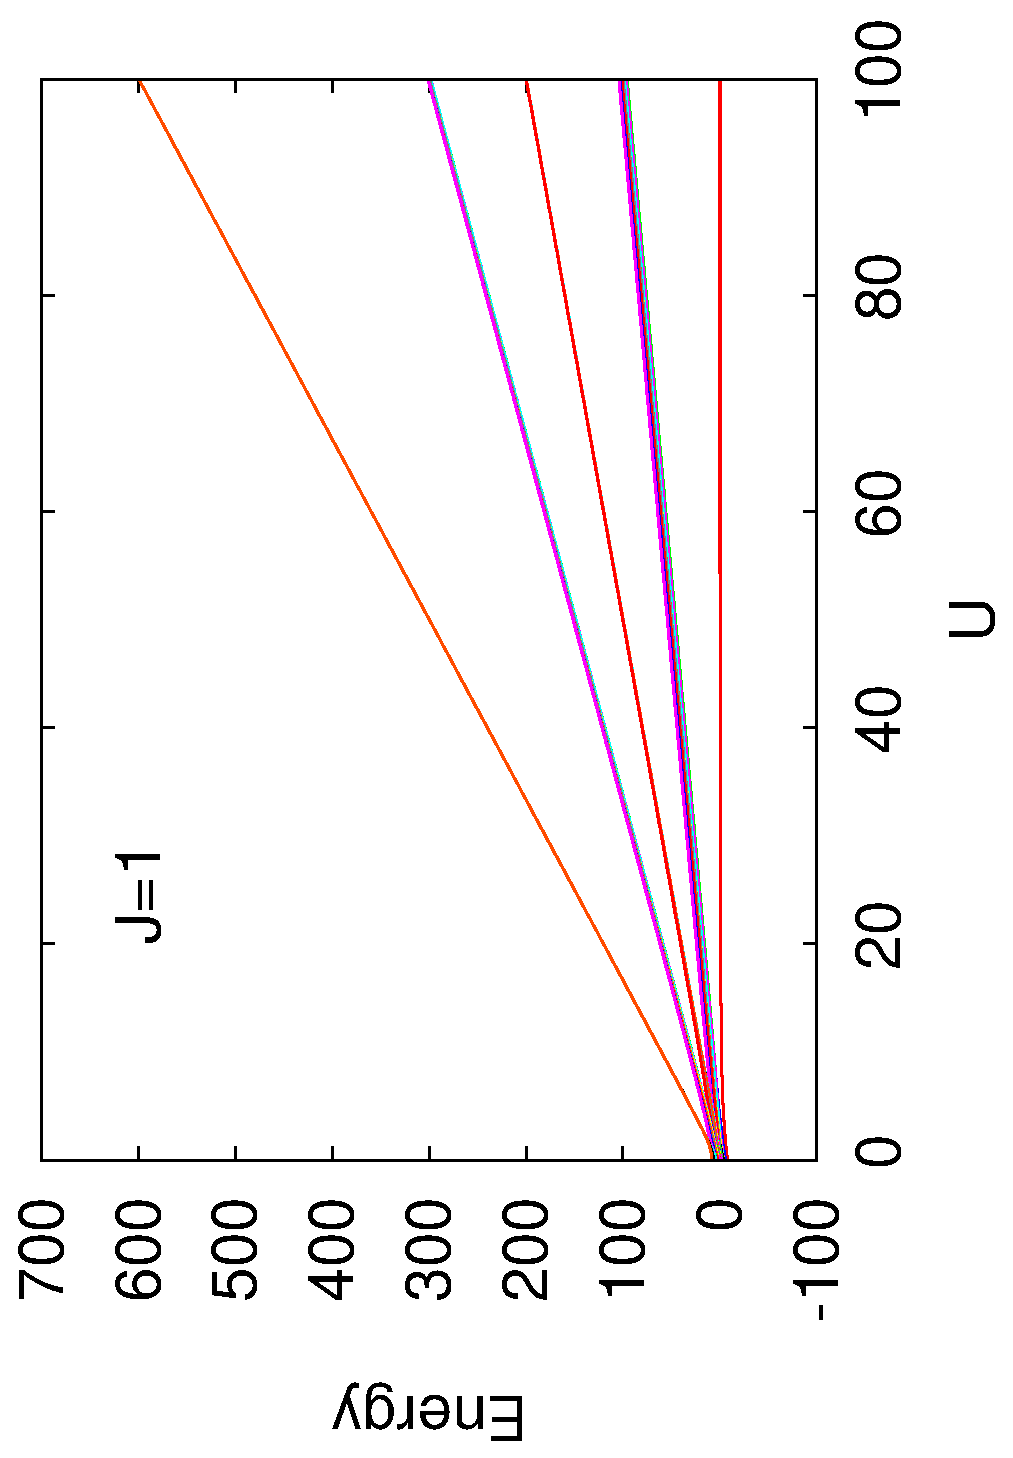
\includegraphics[width=0.35\textwidth, angle=270]{Long_Strong_NL4_NB4_J1.eps}}
  \subfloat[]{ 
   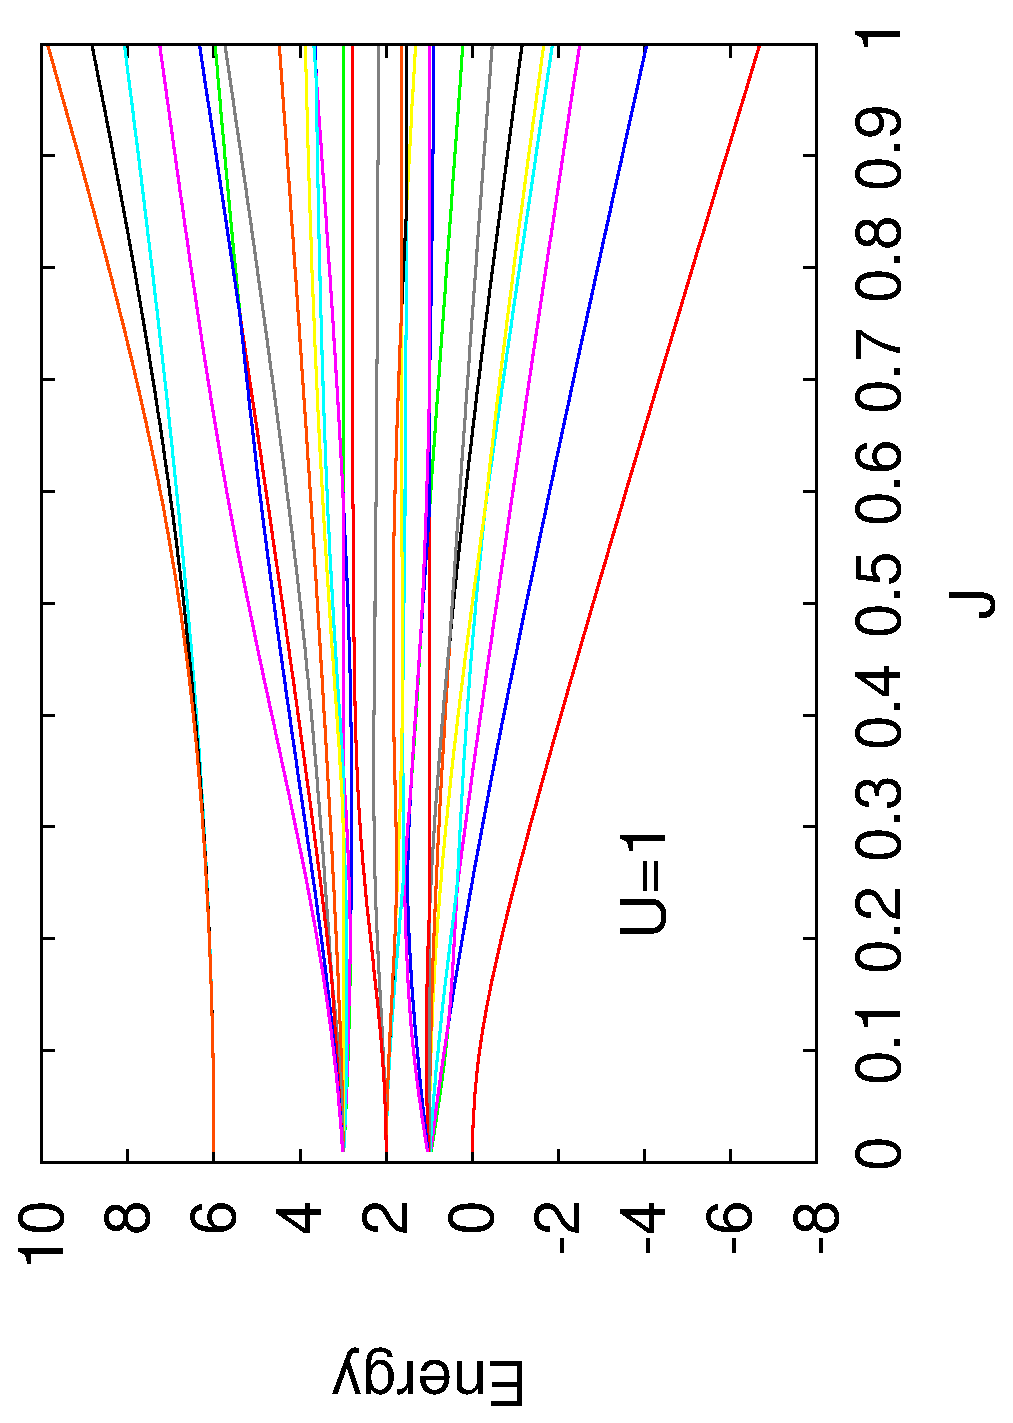
\includegraphics[width=0.35\textwidth, angle=270]{Short_Weak_NL4_NB4_U1.eps}}
  \caption{Espectro del Hamiltoniano para valores de (a) $J=1$, $U$ varía y (b) $U=1$, $J$ varía para $N_L=N_B=4$.}
 \label{f:comparacion}
\end{figure}


En las figuras \ref{f:comparacion} puede observarse que para diferentes valores de $J$ y $U$ existen el mismo número de estados cuando se da la situación para que se esté en el mismo régimen. Además puede verse como en el estado de superfluido hay muchos más estados no degenerados que en el de aislante.

\section{Dinámica del sistema}

En nuestro caso el Hamiltoniano es independiente del tiempo y por tanto podemos calcular evolución temporal desarrollando directamente en la base del espacio de Fock. De manera que el resultado quedaría

\begin{equation}
  \langle\phi(t)|N_k|\phi(t)\rangle=\sum_{i,j}^{D}c_i^*c_j\langle\psi_i|N_k|\psi_j\rangle \cos(\frac{\Delta E_{ij}t}{\hbar})
\end{equation}

donde los $|\psi(t)\rangle$ son los autoestados del Hamiltoniano Bose-Hubbard.

Para un sistema con tres pozos potenciales y 6 bosones con estado inicial preparado de manera que todos se encuentren en el mismo pozo potencial y con suficiente energía para que puedan tunelear, nos encontramos con la evolución dinámica mostrada en la figura \ref{f:dinamica}. En ella se han representado los valores esperados del operador número en cada uno de los pozos potenciales. Sin embargo, cabe destacar que no aparece por ningún lado los datos referentes al segundo pozo potencial. La raíz de este detalle es la condición de contorno periódica que habíamos impuesto: como todos los bosones están en un mismo pozo potencial les es indiferente tunelear hacia la derecha o hacia la izquierda, puesto que en ambos sitios hay el mismo número de bosones y les es energéticamente idéntico. Es decir, el valor esperado del operador número del segundo y tercer pozo potencial están degenerados.


\begin{figure}[h]
  \centering
  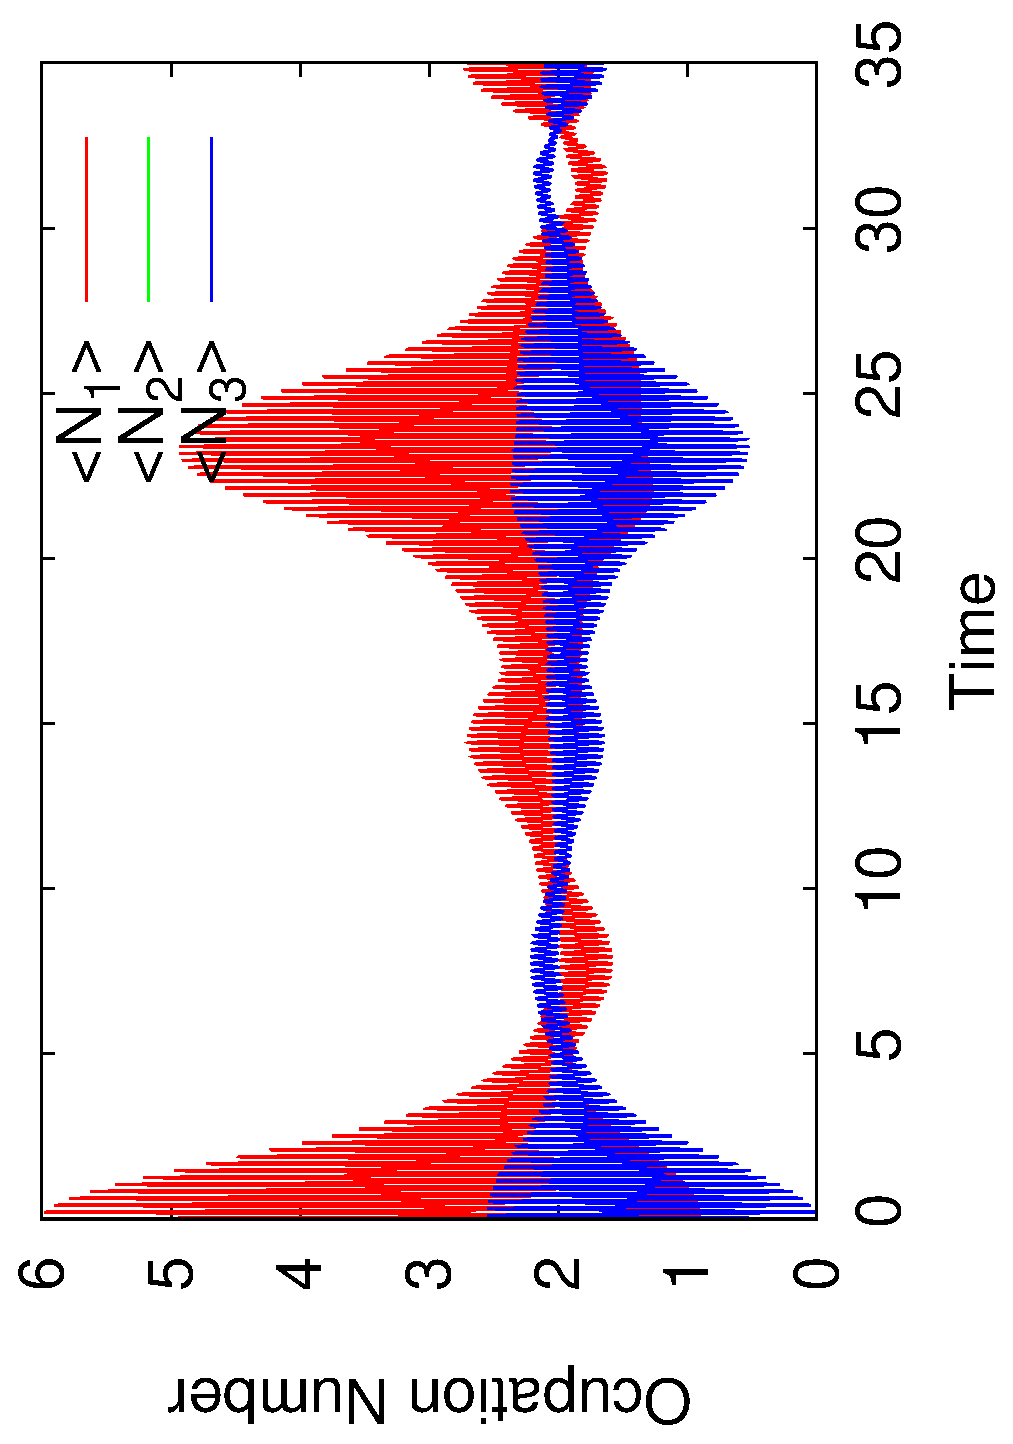
\includegraphics[width=8cm,angle=270]{Prop_600_NL3_NB6_U1_J10.eps}
  \caption{Dinámica del sistema para $N_L=3$, $N_B=6$. Se prepara el sistema con todos los bosones en el primer mínimo. Se les ha dado valores $U=1$ y $J=10$.}
  \label{f:dinamica}
\end{figure}
\noindent


\section{Conclusiones}

En este  pequeño artículo hemos puesto de manifiesto uno de los modelos más sencillos que se pueden encontrar en el campo de los átomos fríos atrapados. Como hemos dicho ya, es un campo que ahora mismo es muy popular e importante para la teconología e información cuántica.

Fijémonos que en esteartículo hemos hablado exclusivamente de la ecuación de Schroedinger independiente del tiempo y de la evolución temporal a lo largo de la red. Pero no hemos hablado en absoluto de la interacción átomo-luz con los rayos láseres. Se puede hacer, y de hecho se hace, excitar a las partículas con otros láseres a un estado diferente, obteniéndose átomos Rydberg. Estos átomos se comportan curiosamente como fermiones aunque sean bosones, y antes de que se produzca la dinámica que aquí hemos visto, se pueden tomar medidas sobre entrelazamiento cuántico bastantes buenas.

Un siguiente paso de este artículo puede ser tratar redes más complejas, de otras geometrías y dimensiones. Así como también se podría hacer variar los diferentes parámetros del Hamiltoniano a lo largo del tiempo y ver si la función de onda colapsaría en algún momento.

Por último, hablar de la dimensión del sistema. En cuántica los sistemas viven dentro del espacio de Hilbert y su dimensión es bastante más alta que en los sistemas cuánticos. Concretamente, en este modelo la dimensión viene dada por

\begin{equation}
  D=\frac{(N_L+N_B-1)!}{(N_L-1)!N_B!}
\end{equation}

De manera que la dimensión de nuestro sistema escala de la forma en la que se indica en la tabla \ref{t:dimension}. De manera que supone un gran esfuerzo computacional resolver sistemas muy grandes de tamaño y de bosones.


\begin{table}[h]
  \centering
  
  \begin{tabular}{|c||c||c|}
    
    \hline
    $N_L$ & $N_B$ & $D$ \\
    \hline
    4 & 4 & 35 \\
    \hline
    6 & 6 & 432 \\
    \hline
    6 & 12 & 6188 \\
    \hline
  \end{tabular}
  \label{t:dimension}
\end{table}


Para terminar, expongo aquí una matriz sobre un tema de estabilidad de matrices usados en ecología, que no tiene nada que ver con el tema, pero sirve como una sgunda tabla para el trabajo.

\begin{equation}
  \left(
  \begin{array}{cccccc}
    0 & \cdots & 0 & -\alpha_{11}^* & \cdots & -\alpha_{1m}^* \\
    \vdots & \ddots & \vdots & \vdots & \ddots & \vdots \\
    0 & \cdots & 0 & -\alpha_{m1}^* & \cdots & -\alpha_{mm}^* \\
    \beta_{11}^* & \cdots & \beta_{1m}^* & 0 & \cdots & 0 \\
    \vdots & \ddots & \vdots & \vdots & \ddots & \vdots \\
    \beta_{m1}^* & \cdots & \beta_{mm}^* & 0 & \cdots & 0 
  \end{array}
  \right)
\end{equation}

Este último se ha hecho como una ecuación.



\bibliography{base_modulo_5}
\bibliographystyle{plain}

\nocite{Smith}
\nocite{Galindo}
\nocite{Sakurai}
\nocite{Laser}
\nocite{Ashcroft}
\nocite{Caos}
\nocite{Yo}

\end{document}
